%************************************************
\chapter{Introduction}\label{ch:introduction}
%************************************************

\lettrine[lines=3]{H}{ello} and welcome to this thesis. It will be very exiting! I bet you won't be able to put it down for days and days and days\dots

%\section{Preliminary Definitions and Assumptions}

\section{Methodology}

In this thesis we follow closely a methodology called \emph{sociologically inspired computing}~\citep{Jones2013}. This is a method for the design of socio-technical systems from the analysis of social and organisational concepts. Built upon the synthetic method underlying research in artificial societies and artificial life~\citep{Steels1994}, the formalisation of social relations in multi-agent systems~\citep{Neville2004}, and other attempts to apply ideas from the social sciences to the design of computational systems~\citep{Edmonds2005}, it provides a series of steps to go from an observed social phenomenon to an observed performance of a derived computer model under controlled experimentation conditions. These steps are illustrated in \autoref{fig:sic}.

\begin{figure}
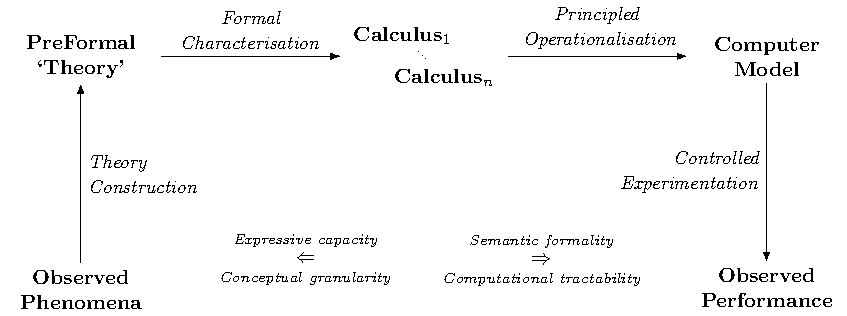
\includegraphics[width=\linewidth]{gfx/sic}
\caption[Methodology for sociologically inspired computing.]{Methodology for sociologically inspired computing~\citep{Jones2013}.}\label{fig:sic}
\end{figure}

% TODO Interleave what we actually do.
We begin with an observed phenomenon, for example, from the social sciences, a human social, legal, or organisational system. The process of \emph{Theory Construction} generates a \emph{PreFormal Theory}, usually expressed in a natural language. \emph{Formal Characterisation} creates a specification of this theory in a calculus of some kind, where `calculus' is meant to be any system of calculation or computation based on the manipulation of symbolic representations. This calculus is then embedded in a computer model in the \emph{Principled Operationalisation} step. This computer model enables simulations that can include both implementations of individual agents, and/or treatment of large populations. Through \emph{Controlled Experimentation} with this computer model we can observe the performance of the model.

Through our use of this methodology we have two major contributions to the \emph{Principled Operationalisation} and \emph{Controlled Experimentation} steps. The platform Presage2~\citep{Macbeth2014} which enables both of these steps, and a rule engine for Electronic Institution which enables rapid operationalisation of common concepts from Electronic Institutions, with flexibility to accommodate further rules from the calculus. These contributions are presented in \autoref{ch:presage} and \autoref{ch:droolseinst} respectively.
